\documentclass[12pt,a4paper]{report}
\usepackage[utf8]{vietnam}
\usepackage{amsmath}
\usepackage{amsfonts}
\usepackage{amssymb}
\usepackage{makeidx}
\usepackage{graphicx}
\usepackage[left=3.50cm, right=2.00cm, top=3.50cm, bottom=3.00cm]{geometry}
\usepackage{scrextend}
\changefontsizes{13pt}
\usepackage{fancyhdr}
\pagestyle{fancy}
\lhead{\textit{CHỦ ĐỀ TỐI ƯU}}
\chead{}
\rhead{\textit{GVHD: PGS.TS ĐỖ ĐỨC THUẬN}}
\lfoot{\textit{SVTH: HOÀNG THANH LƯU}}
\cfoot{\thepage}
\rfoot{\textit{TOÁN TIN K61}}
\renewcommand{\headrulewidth}{0.4pt}
\renewcommand{\footrulewidth}{0.4pt}
\begin{document}
	\begin{center}
		\textbf{STOCHASTIC PROGRAMMING}
	\end{center}
	\tableofcontents
	\chapter{Các khái niệm cơ bản}
	
	
	
	
	%%%%%%%%%%%%%%%%%%%%%%%%%%%%%%%%%
	\chapter{Hệ thống động}
	\section{Nguyên tắc Bellman}
	Như đã thảo luận trong Chương 1, các vấn đề tối ưu hóa có thể có nhiều loại khác nhau. Các sự khác biệt có thể được tìm thấy trong mục tiêu, tức là tối thiểu hóa hoặc tối đa hóa, trong các ràng buộc, tức là bất đẳng thức hoặc bất đẳng thức và các biến tự do hoặc không âm, và trong các tính chất toán học của các hàm liên quan đến mục tiêu hoặc các ràng buộc. Chúng ta đã gặp các hàm tuyến tính trong Mục 1.6, phi tuyến trong Mục 1.7 và thậm chí cả hai hàm trong Mục 1.3. Mặc dù chúng có những khác biệt, tất cả những vấn đề này có thể được trình bày dưới dạng thống nhất
	\begin{equation}
		\max\{F(x_1,x_2,...x_n) | x \in X\} \nonumber
	\end{equation}
	Ở đây $X$ là tập các phương án chấp nhận được mà chúng ta cố gắng tối đa hóa, hoặc thỉnh thoảng là tối thiểu hóa hàm mục tiêu đã cho $F$.
	\newline
	Cài đặt chung này cũng bao gồm một lớp quyết định hơi đặc biệt
	các vấn đề. Chúng được minh họa trong Hình 2.1.
	\newline Hãy xem xét một hệ thống được kiểm tra ở nhiều giai đoạn. Ví dụ trong Hình 1 có 4 giai đoạn. Điều này được nhìn thấy từ thực tế là có bốn cột. Giả sử rằng ở bất kỳ giai đoạn nào, hệ thống có thể ở một trong số rất nhiều trạng thái. Trong Hình 2.1, có bốn trạng thái có thể có trong mỗi giai đoạn, được biểu thị bằng bốn trạng thái chấm trong mỗi cột. Ngoài ra, ở bất kì giai đoạn nào (ngoại trừ giai đoạn cuối cùng) phải được thực hiện mà có thể sẽ có ảnh hưởng đến trạng thái hệ thống ở giai đoạn tiếp theo. Kèm theo quyết định là một sự trở lại ngay lập tức (hoặc cách khác một chi phí ngay lập tức) \textit{(? - Attached to the decision is an immediate return (or else
	an immediate cost))}. Trong Hình 2.1, ba mũi tên ở phần bên phải của hình chỉ ra rằng trong ví dụ này có ba quyết định khả thi: Một mang đến chúng ta ở trạng thái thấp hơn trong giai đoạn tiếp theo, một giữ chúng ta ở trạng thái tương tự và một đưa chúng ta đến một trạng thái cao hơn (Chúng ta phải cho rằng nếu chúng ta ở mức cao nhất hoặc trạng thái thấp nhất có thể sau đó chỉ có hai quyết định là có thể thực hiện). Đưa ra ban đầu trạng thái của hệ thống, mục tiêu tổng thể là tối đa hóa hoặc tối thiểu hóa một số chức năng nhất định của lợi nhuận ngay lập tức cho tất cả các giai đoạn và nêu hệ thống đi qua như là kết quả của các quyết định của chúng ta. Một cách chính thức được mô tả như sau: 
	\newline
	\begin{figure}[h]
		\centering
		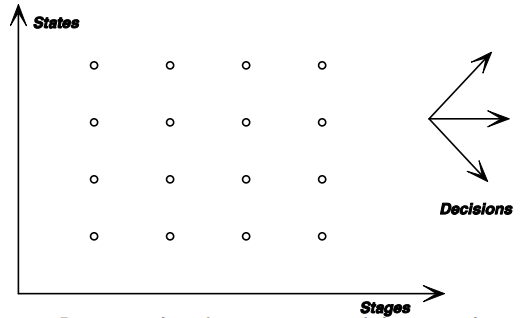
\includegraphics[scale=.8]{hinh1.png}
		\caption{Thiết lập cơ bản cho một chương trình động với bốn trạng thái, bốn giai đoạn và ba quyết định có thể.}                  
	\end{figure}

	\begin{list}{}{%
			% độ rộng biên trái
			\setlength{\leftmargin}{1.2in}
			% độ rộng phần chứa nhãn
			\setlength{\labelwidth}{1.2in}
			% khoảng trắng ngang giữa nhãn và text
			\setlength{\labelsep}{0.0in}
			% khoảng trắng dọc giữa hai item
			\setlength{\parsep}{5pt plus 1pt minus 0pt}
			% khoảng trắng dọc giữa hai item
			\setlength{\itemsep}{7pt plus 1pt minus 0pt}
			% khoảng trắng dọc trước và sau môi trường list
			\setlength{\topsep}{10pt plus 1pt minus 0pt}
		}
		\item[$t$\hfill]
		 các giai đoạn, $t = 1, \cdots, T$,		 
		\item[$Z_t$\hfill] các trạng thái ở giai đoạn $t$,		
		\item[$x_t$\hfill]quyết định đưa ra ở giai đoạn $t$, (nói chung tùy thuộc vào trạng thái $z_t$), 		
		\item[$G_t(z_t, z_t)$ \hfill]  sự chuyển đổi (hoặc chuyển đổi) của hệ thống từ trạng thái $z_t$
		và quyết định được đưa ra ở giai đoạn $t$ vào trạng thái $z_{t + 1}$ ở lần tiếp theo, tức là $z_{t+1} = G_t(z_t, x_t)$, 		
		\item[$r_t(z_t, x_t)$\hfill]  lợi nhuận ngay lập tức nếu ở giai đoạn $t$ hệ thống ở trạng thái $z_t$ và
		quyết định $x_t$ được đưa ra, 		
		\item[$F$\hfill] mục tiêu tổng thể, được đưa ra bởi $F(r_1(z_1,x_1), \cdots, r_T(z_T, x_T))$, và 
		\item[$X_t(z_t)$\hfill]tập hợp các quyết định khả thi ở giai đoạn $t$, (có thể phụ thuộc vào
		trạng thái $z_t$),			
	\end{list}						
	Vấn đề của chúng ta có thể được nêu là
	\begin{equation}
		\max\{F(r_1(z_1, x_1), \cdots, r_T(z_T, x_T))|x_t \in X, t = 1, \cdots, T\}
		\nonumber
	\end{equation}
	Bởi vì ta có mỗi quan hệ $z_{t+1} = G_t(z_t, x_t)$, hàm mục tiêu có thể được viết lại dưới dạng $\Phi (z_1, x_1, x_2, \cdots, x_T)$. Để có được ý tưởng về các cấu trúc có thể có mà chúng ta có thể đối mặt, chúng ta hãy xem lại ví dụ trong Hình 2.1. Mục đích của ví dụ này không phải là thực tế, mà là để minh họa một vài điểm. Một vấn đề thực tế hơn sẽ được thảo luận trong phần tiếp theo.
	\newline
	\newline
	\textbf{Ví dụ 2.1} Giả sử rằng các giai đoạn là năm và hệ thống được kiểm tra
	hàng năm, sao cho ba giai đoạn tương ứng với ngày 1 tháng 1 của năm thứ nhất, thứ hai và thứ ba và ngày 31 tháng 12 của năm thứ ba. Giả sử thêm rằng bốn cấp độ khác nhau được phân biệt là các trạng thái cho hệ thống, tức là ở bất kỳ giai đoạn nào, người ta có thể quan sát trạng thái $z_t$ = 1; 2; 3 hoặc 4. Cuối cùng, tùy thuộc vào trạng thái của hệ thống trong giai đoạn 1; 2 và 3; một trong những quyết định sau đây có thể được đưa ra: 
	$$
	x_t = \begin{cases}
	1, \quad \text{ dẫn đến sự trở lại ngay lập tức } r_t = 2,\\ 
	0, \quad\text{ dẫn đến sự trở lại ngay lập tức } r_t = 1,\\
	-1, \quad\text{dẫn đến sự trở lại ngay lập tức } r_t = -1.
	\end{cases}
	$$
	Việc chuyển từ giai đoạn này sang giai đoạn tiếp theo được đưa ra bởi $$ z_{t+1} = z_t + x_t $$
	Lưu ý rằng, vì $z_t \in \{1,2,3,4\}$ cho tất cả $t$, chúng ta có $x_t = 1$ ở trạng thái $z_t = 4$ và $x_t = -1$ ở trạng thái $z_t = 1$ là không khả thi, và do đó bị loại trừ. Cuối cùng, giả sử rằng không có quyết định nào trong giai đoạn cuối T = 4. Tuy nhiên, có những khoản hoàn trả ngay lập tức	$$
	r_T = \begin{cases}
	-2, \quad \text{nếu } z_T = 4,\\
	-1, \quad \text{nếu } z_T = 3,\\
	1, \quad \text{nếu } z_T = 2,\\
	2, \quad \text{nếu } z_T = 1.
	\end{cases}$$
	\nonumber	  
	Để giải $\max F(r_1, \cdots, r_4)$, chúng ta phải sửa mục tiêu tổng thể F là một hàm trả về ngay lập tức $r_1, r_2, r_3, r_4$. Để chứng minh các tác động có thể có của các thuộc tính của $F$ đối với quy trình giải pháp, chúng ta chọn hai biến thể:
	
	\begin{itemize}
		\item[(a)] Cho $$F(r_1,\cdots, r_4) := r_1 + r_2 + r_3 + r_4 $$ và giả sử rằng trạng thái ban đầu là $z_1 = 4$. Điều này được minh họa trong Hình 2.2, có cùng cấu trúc như Hình 2.1. Sử dụng hình, chúng ta có thể kiểm tra xem một chính sách tối ưu (tức là chuỗi các quyết định), là $x_1 = x_2 = x_3 = 0$ giữ chúng ta trong $z_t = 4$ với mọi $t$ với giá trị tối ưu $F (r_1,\cdots,r_4) = 1 + 1 + 1 - 2 = 1.$ Chúng ta có thể xác định chính sách tối ưu này lặp đi lặp lại như sau. Đầu tiên, chúng ta xác định quyết định cho từng trạng thái trong giai đoạn 3 bằng cách xác định $$f^*_3(z_3) := \max_{x_3}[r_3(z_3,x_3) + r_4(z_4)]$$
		
		\begin{figure}[h]
		\centering
		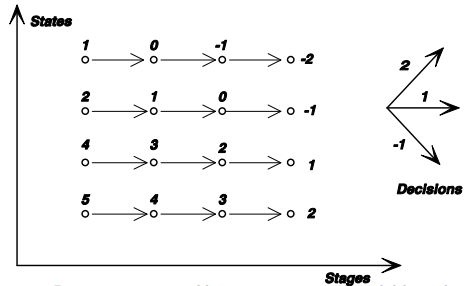
\includegraphics[scale=.85]{hinh2.png}
		\caption{Chương trình động: thành phần phụ gia. Các đường liền nét cho thấy
			kết quả của đệ quy ngược.}
		\end{figure}
		
		cho $z_3 = 1, \cdots, 4$,  và $z_4 = G_3 (z_3, x_3) = z_3 + x_3$. Ví dụ: nếu chúng ta ở trạng thái 2, tức là $z_3 = 2$, chúng ta có ba tùy chọn, đó là -1, 0 và 1. Nếu $x_3 = 1$, chúng ta nhận được thu nhập ngay lập tức là 2 và giá trị cuối cùng là -1, kể từ khi quyết định này sẽ dẫn đến $z_4 = 2 + 1 = 3$. 
		Tùy chọn thứ hai là để $x_3 = 0$, mang lại thu nhập ngay lập tức là 1 và giá trị cuối cùng là 1. 
		Khả năng thứ ba là để $x_3 = -1$, mang lại thu nhập -1 và 1. Do đó, tổng thu nhập lần lượt là 1, 2 và 0, vì vậy lựa chọn tốt nhất là để $z_3 = 0$. Điều này được minh họa trong hình bằng cách đặt một mũi tên từ trạng thái 2 ở giai đoạn 3 đến trạng thái 2 ở giai đoạn 4. Với "$(z_3 = i) \to (x_3, f^*_3)$" chỉ ra rằng ở trạng thái $z_3 = i$ quyết định tối ưu là $x_3$ và tổng thu nhập trước mắt và cuối cùng là $f_3^*$, chúng ta có thể lặp lại quy trình trên cho từng trạng thái trong giai đoạn 3 để có được $(z_3 = 1 ) \to (0, 3), (z_3 = 2) \to (0, 2); (z_3 = 3) \to (0, 0); (z_3 = 4) \to (0, -1)$. Tất cả điều này được minh họa trong Hình 2.2, bằng cách thêm các giá trị $f^*_3$ phía trên các nút trạng thái trong giai đoạn 3.
		
		Khi $f_3^*(z_3)$ được biết đến với tất cả các giá trị của $z_3$, chúng ta có thể chuyển sang giai đoạn 2 và xác định tương tự $$f_2^*(z_2):=\max_{x_2}[r_2(z_2, x_2) + f^*_3(z_3)]$$ với $z_3 = G_2(z_2, x_2) = z_2 + x_2$. 
		Điều này mang lại $f_2^*(1) = 4, f_2^*(2)=3, f^*_2(3) = 1$ và $f^*_2(4) = 0.$ Điều này một lần nữa được minh họa trong Hình 2.2, cùng với các quyết định tối ưu tương ứng.\\
		Cuối cùng, với $z_1 = 4$, vấn đề có thể được thực thi lại là $$f_1^*(z_1):=\max_{x_1}[r_1(z_1, x_1) + f^*_2(z_2)]$$ với $z_2 = G_1(z_1, x_1) = z_1 + x_1$. Điều này ngay lập tức mang lại $f_1^*(z_1) = 1$ cho $x_1 = 0$.\\
		
		Trong ví dụ đơn giản này, dễ dàng nhận thấy rằng $f_1^*(z_1)$trùng với
		giá trị tối ưu của $F = (r_1, \cdots, r_4)$, với trạng thái ban đầu $z_1$, để vấn đề có thể được giải quyết với đệ quy ngược ở trên. (Đệ quy được gọi là lùi vì chúng ta bắt đầu trong giai đoạn cuối và di chuyển ngược thời gian, kết thúc ở giai đoạn 1.)\\
		Lưu ý rằng một cách khác để giải quyết vấn đề này sẽ là liệt kê tất cả các chuỗi quyết định có thể có. Đối với vấn đề nhỏ này, đó sẽ là một nhiệm vụ khá đơn giản. Nhưng đối với các vấn đề lớn hơn, cả về trạng thái và giai đoạn (đặc biệt là khi cả hai đều đa chiều), dễ dàng nhận thấy rằng điều này sẽ trở thành một nhiệm vụ bất khả thi. Việc giảm từ liệt kê đầy đủ tất cả các chuỗi quyết định có thể sang việc tìm ra quyết định tối ưu ở tất cả các trạng thái là lý do chính để quan tâm đến đệ quy lạc hậu và nói chung hơn là vì quan tâm đến lập trình động. 
		
		\item[(b)] Như một sự thay thế, chúng ta có thể sử dụng phép nhân để có được $$F(r_1, \cdots, r_4) := r_1r_2r_3r_4$$ và thực hiện đệ quy ngược như trên, thu được Hình 2.3. Với $$f^*_t(z_t) := \max_{x_t}[r_t(z_t, x_t)f^*_{t+1} (z_{t+1})]$$cho $t = 3,2,1$, với $z_{t+1} = G_t(z_t, x_t) = z_t + x_t$ và $f_4^*(z_4) = r_4(z_4)$, chúng ta nên lấy $f_1^*(z_1 = 4) = 1$ với chính sách tối ưu hóa (0,0,-1). Tuy nhiên, chính sách (-1,1,0) mang lại $F(r_1, \cdots, r_4) = 4.$ Do đó đệ quy ngược không mang lại kết quả tối ưu giải pháp khi lợi nhuận được tính theo cách nhân.
		
		\begin{figure}[h]
			\centering
			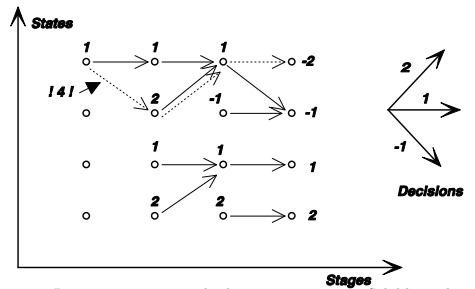
\includegraphics[scale=.9]{hinh3.png}
			\caption{Chương trình động: thành phần nhân. Đường liền nét cho thấy
				kết quả của đệ quy ngược (với $z_1 = 4$), trong khi đường chấm chấm hiển thị chuỗi quyết định tối ưu.}
		\end{figure} 
		\end{itemize}	
		
		Trong ví dụ trên, chúng ta đã có $$F(r_1(z_1,x_1),\cdots, r_T(z_T, x_T)) = r_1(z_1, x_1) \oplus r_2(z_2, x_2) \oplus \cdots \oplus r_T(z_T, x_T), $$
		trong đó thao tác phép toán $\oplus$ được chọn là phép cộng trong trường hợp (a) và phép nhân trong trường hợp (b). Đối với đệ quy lạc hậu, chúng ta đã sử dụng cái gọi là phân tách của F. Nghĩa là, tồn tại hai hàm số $\varphi_1, \psi_2$ sao cho
		\begin{eqnarray}
		F(r_1(z_1,x_1), \cdots, r_T(z_T, x_T))   = \varphi_1(r_1(z_1, x_1), \psi_2(r_2(z_2, x_2), \cdots, r_T(z_T, x_T))).
		\end{eqnarray}
		\\
		\noindent
		Hơn nữa, chúng ta tiến hành như thể các mối quan hệ sau đây được tổ chức \begin{eqnarray}
			\max\{F(r_1(z_1, x_1),\cdots, r_T(z_T, x_T)) | x_t \in X_T, t = 1, \cdots T\}  \\ \nonumber = \max_{x_1 \in X_1}[\varphi_1(r_1(z_1, x_1), \max_{x_2 \in X_2, \cdots, x_T \in X_T}\psi(r_2(z_2, x_2), \cdots, r_T(z_T, x_T)))].
		\end{eqnarray}  
		Mối quan hệ này là tương đương chính thức của nguyên tắc tối ưu nổi tiếng, được Bellman thể hiện như sau (trích dẫn)
		\\\\
		\textbf{Định lý 2.1} \textit{"Một chính sách tối ưu có đặc điểm là bất kể trạng thái ban đầu và quyết định ban đầu là gì, các quyết định còn lại phải tạo thành một chính sách tối ưu liên quan đến trạng thái từ quyết định đầu tiên."}
		\\\\		
		Như chúng ta đã thấy trong Ví dụ 2.1, nguyên tắc này được áp dụng nhiều lần trong đệ quy ngược, đã đưa ra giải pháp tối ưu cho trường hợp (a) nhưng không áp dụng cho trường hợp (b). Lý do cho điều này là vì, mặc dù phép toán $\oplus$ có thể tách rời theo nghĩa của (2.1), nhưng điều này không đủ để đảm bảo rằng việc áp dụng lặp lại nguyên tắc tối ưu (tức là thông qua đệ quy ngược) sẽ mang lại một chính sách tối ưu. Một điều kiện đủ theo đó nguyên tắc tối ưu nắm giữ liên quan đến tính đơn điệu nhất định của phép toàn $\oplus$. Chính xác hơn, chúng ta có những điều sau đây.\\\\
		\textbf{Định lý 2.2} \textit{Nếu $F$ thỏa mãn điều kiện phân tách (2.1) và nếu $\varphi_1$ không đơn điệu trong $\psi_2$ cho mỗi $r_1$ thì nguyên tắc tối ưu (2.2) được giữ vững.}\\\\
		\textit{Chứng minh}
		\begin{eqnarray}
		\max_{\{x_t \in X_t, t \geq 1\}} \varphi_1(r_1(z_1, x_1), \psi_2(r_2(z_2,x_2),\cdots, r_T(z_T, x_T))) \nonumber \\  \geq \varphi_1(r_1(z_1, x_1), \max_{\{x_t \in X_t, t \geq 2\}}[\psi_2(r_2(z_2, x_2), \cdots, r_T(z_T, x_T))]), \nonumber
		\end{eqnarray}  
		cho tất cả $x_1$. Do đó, điều này cũng đúng khi phía bên phải của bất đẳng thức này được tối đa hóa đối với $x_1$. Mặt khác, rõ ràng là
			\begin{eqnarray}
		\max_{\{x_t \in X_t, t \geq 2\}}\psi_2(r_2(z_2,x_2),\cdots, r_T(z_T, x_T)) \nonumber \\  \geq \psi_2(r_2(z_2, x_2), \cdots, r_T(z_T, x_T)), \forall x_t \in X_t, t \geq 2. \nonumber
		\end{eqnarray} Do đó, bằng tính đơn điệu giả định của $\psi_1$ đối với $\psi_2$, ta có 	\begin{eqnarray}
 		\varphi_1(r_1(z_1, x_1), \max_{\{x_t \in X_t, t \geq 2\}}\psi_2(r_2(z_2, x_2), \cdots, r_T(z_T, x_T)) \nonumber\\ \geq \varphi_1(r_1(z_1,x_1), \psi_2(r_2(z_2,x_2), \cdots, r_T(z_T, x_T)))  \forall x_t \in X_t, t \geq 1. \nonumber
		\end{eqnarray} Lấy tối đa đối với $x_t, t \geq 2$, ở phía bên phải của bất đẳng thức và tối đa hóa sau đó cả hai bên đối với $x_1 \in X1$ cho thấy nguyên tắc tối ưu (2.2) được giữ vững. 
		\\\\Không cần phải nói, tất cả các vấn đề được Bellman xem xét trong cuốn sách đầu tiên của ông về lập trình động thỏa mãn đề xuất này. Trong trường hợp (b) của ví dụ trên,	
		tuy nhiên, sự đơn điệu không giữ được. Lý do là vì khi  $\oplus$ là tích, các yếu tố có thể tiêu cực (nghĩa là lợi nhuận tức thời âm), sự đơn điệu cần thiết bị mất. Mặt khác, khi mà $\oplus$ là tổng, 
		sự đơn điệu cần thiết luôn được thỏa mãn.\\\\ Chúng ta hãy thêm rằng nguyên tắc tối ưu áp dụng cho một loại vấn đề rộng hơn nhiều so với dường như là trường hợp từ bản phác thảo ngắn gọn này. Chẳng hạn, nếu đối với nhiều trạng thái, chúng ta biểu thị bằng $\rho_t$ thì vectơ có thành phần thứ $i$ là $r_t$ trả về ngay lập tức $(z_t = i)$ và nếu chúng ta xác định phép toán thành phần $\oplus$ sao cho, với ma trận dương $S$ (tức là tất cả các phần tử của $S$ không âm), $$\rho_t \oplus \rho_{t+1} = \rho_t + S\rho_{t+1}, t = 1, \cdots, T-1$$ sau đó tính đơn điệu được giả định cho Định lý 2.2 ngay sau đó. Trường hợp này là khá phổ biến trong các ứng dụng. $S$ là ma trận chuyển tiếp, có nghĩa là một phần tử $s_{ij}$ đại diện cho xác suất vào trạng thái $j$ ở giai đoạn $t + 1$, với điều kiện là hệ thống ở trạng thái $i$, giai đoạn $t$. Lặp lại thành phần trên cho $T-1, T-2, \cdots, 1$, chúng ta nhận được $F(\rho_1, \cdots, \rho_T)$ là vectơ của tổng lợi nhuận dự kiến. Thành phần thứ $i$ mang lại lợi nhuận tổng thể dự kiến nếu hệ thống bắt đầu từ trạng thái $i$ ở giai đoạn 1. 
	\section{Quy hoạch động}
		Mục đích của phần này là xem xét các khía cạnh nhất định của lĩnh vực lập trình động. Ví dụ chúng ta đã xem xét trong phần trước là một ví dụ về vấn đề lập trình động. Nó sẽ không đại diện cho một mô tả công bằng về toàn bộ lĩnh vực, nhưng chúng tôi sẽ tập trung vào các khía cạnh hữu ích trong bối cảnh của chúng tôi. Phần này sẽ không xem xét tính ngẫu nhiên. Điều đó sẽ được thảo luận sau.\\\\
		Chúng ta sẽ quan tâm đến lập trình động như một phương tiện để giải quyết các vấn đề phát triển theo thời gian. Ví dụ điển hình là lập kế hoạch sản xuất theo nhu cầu khác nhau, mở rộng công suất để đáp ứng nhu cầu ngày càng tăng và lập kế hoạch đầu tư trong lâm nghiệp. Lập trình động cũng có thể được sử dụng để giải quyết các vấn đề không có tính chất tuần tự. Những vấn đề như vậy sẽ không được xử lý trong văn bản này.\\\\
		Các khái niệm quan trọng trong lập trình động là chân trời thời gian, biến trạng thái, biến quyết định, hàm trả về, hàm trả về tích lũy, lợi nhuận tích lũy tối ưu và hàm chuyển tiếp. Chân trời thời gian đề cập đến số lượng giai đoạn (khoảng thời gian) trong vấn đề. Các biến trạng thái mô tả trạng thái của hệ thống, ví dụ như năng lực sản xuất hiện tại, tuổi hiện tại và phân bố loài trong một khu rừng hoặc số tiền người ta có trong các tài khoản khác nhau trong một ngân hàng. Các biến quyết định là các biến dưới một điều khiển. Họ có thể đại diện cho các quyết định xây dựng nhà máy mới, để cắt một lượng gỗ nhất định hoặc chuyển tiền từ tài khoản ngân hàng này sang tài khoản khác. Hàm chuyển đổi cho thấy các biến trạng thái thay đổi như một hàm của các quyết định. Đó là, chức năng chuyển tiếp quyết định trạng thái sẽ là kết quả của sự kết hợp giữa trạng thái hiện tại và các quyết định hiện tại. Ví dụ, chức năng chuyển đổi có thể cho thấy rừng thay đổi như thế nào trong giai đoạn tiếp theo do tình trạng hiện tại và các quyết định cắt giảm, số tiền trong ngân hàng tăng lên, hoặc năng lực sản xuất sẽ thay đổi như thế nào do kết quả của nó quy mô hiện tại, đầu tư (và phá hủy). Hàm trả về hiển thị lợi nhuận ngay lập tức (chi phí hoặc lợi nhuận) là kết quả của việc đưa ra quyết định cụ thể trong một trạng thái cụ thể. Các hàm trả về tích lũy cho thấy hiệu ứng tích lũy, từ nay đến hết chân trời thời gian, liên quan đến một quyết định cụ thể trong một trạng thái cụ thể. Cuối cùng, lợi nhuận tích lũy tối ưu cho thấy giá trị của việc đưa ra quyết định tối ưu dựa trên hàm trả về tích lũy, hay nói cách khác, lợi nhuận tốt nhất có thể đạt được từ trạng thái hiện tại cho đến khi kết thúc thời gian.\\\\
		\textbf{Ví dụ 2.2} Hãy xem xét vấn đề đầu tư đơn giản sau đây, trong đó rõ ràng là nguyên tắc Bellman nắm giữ. Chúng tôi có một số tiền $S_0$ trong tài khoản ngân hàng, được gọi là tài khoản $B$. Chúng tôi sẽ cần tiền hai năm kể từ bây giờ và hôm nay là ngày đầu tiên của tháng một. Nếu chúng tôi để lại tiền trong tài khoản, chúng tôi sẽ phải đối mặt với lãi suất 7 \% trong năm đầu tiên và 5 \% trong năm thứ hai. Bạn cũng có tùy chọn chuyển tiền vào tài khoản $A$. Bạn sẽ phải đối mặt với lãi suất 10\% trong năm đầu tiên và 7\% trong năm thứ hai. Tuy nhiên, có một khoản phí cố định là 20 mỗi năm và một khoản phí là 10 mỗi lần chúng tôi rút tiền từ tài khoản A. Khoản phí cố định được khấu trừ vào tài khoản vào cuối năm, trong khi các khoản phí rút tiền được khấu trừ ngay lập tức. Câu hỏi đặt ra là: Chúng ta nên chuyển tiền vào tài khoản $A$ trong năm đầu tiên, năm thứ hai hay cả hai năm? Trong mọi trường hợp, tiền còn lại trong tài khoản $A$ vào cuối năm thứ hai sẽ được chuyển vào tài khoản $B$. Mục tiêu là giải quyết vấn đề cho tất cả $S_0> 1000$ ban đầu. Hình 2.4 minh họa ví dụ.
		
		\begin{figure}[h]
			\centering
			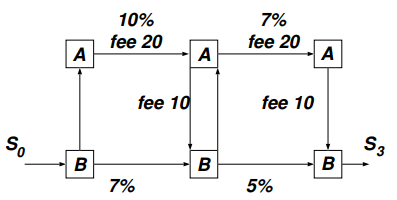
\includegraphics[scale=1]{hinh4.png}
			\caption{
				Mô tả đồ họa của một vấn đề đầu tư đơn giản.}
		\end{figure} \noindent Lưu ý rằng tất cả các khoản đầu tư sẽ dẫn đến trường hợp tài sản tăng lên và sẽ không bao giờ có lãi khi chia tiền giữa các tài khoản (Tại sao?). \\\\Trước tiên chúng ta hãy xác định các biến trạng thái hai chiều $z_t = (z_t^1, z_t^2)$. Biến trạng thái đầu tiên, $z_t^1$, đề cập đến tên tài khoản ($A$ hoặc $B$); biến trạng thái thứ hai, $z_t^2$, đề cập đến số tiền $S_t$ trong tài khoản đó. Vậy $z_t = (B, S_t)$ đề cập đến trạng thái có số tiền $S_t$ trong tài khoản $B$ ở giai đoạn $t$. Quyết định là nơi để đặt tiền cho khoảng thời gian tiếp theo. Nếu $x_t$ là biến quyết định của chúng tôi thì $x_t \in \{A, B\}$. Hàm chuyển đổi sẽ được ký hiệu là $G_t (z_t, x_t)$ và được xác định thông qua lãi suất và phí. Nó cho thấy những gì sẽ xảy ra với tiền trong một năm, dựa trên số tiền hiện tại, số tiền đó là bao nhiêu và nơi nào được đặt tiếp theo. Vì không gian trạng thái có hai phần tử, nên hàm $G_t$ có hai giá trị. Ví dụ $$z_{t+1}^1= G_t^1 \begin{pmatrix}
		\begin{pmatrix}
			A\\S_t
		\end{pmatrix},A
		\end{pmatrix} = A , \qquad \qquad z_{t+1}^2 =  	G_t^2 \begin{pmatrix}
		\begin{pmatrix}
		A\\S_t
		\end{pmatrix},A
		\end{pmatrix} = S_t \times 1.07 - 20.$$ Các hàm trả về tích lũy sẽ được ký hiệu là $f_t(z_t^1, z_t^2, x_t)$. Họ
		mô tả số tiền $z^2_ t$ trong tài khoản $z_t^1$ sẽ tăng lên như thế nào, cho đến cuối thời gian, nếu tiền được đưa vào tài khoản $x_t$ trong giai đoạn tiếp theo và các quyết định tối ưu được đưa ra sau đó. Vì vậy, nếu $f_1 (A, S_1, B) = \overline{S}$, chúng ta biết rằng trong giai đoạn 1 (tức là vào cuối giai đoạn 1), nếu chúng ta có $S_1$ trong tài khoản $A$ và sau đó chuyển nó sang tài khoản $B$, chúng ta sẽ còn lại $S_3 = \overline{S}$ trong tài khoản $B$ ở cuối thời gian, do chúng ta đưa ra quyết định tối ưu ở tất cả các giai đoạn sau giai đoạn 1. Bằng cách tối đa hóa tất cả các quyết định có thể, chúng ta thấy lợi nhuận tích lũy tối ưu $f_t^* (z_t^1, z_t^2)$ cho một trạng thái nhất định. Ví dụ, $$f^*_1(A, S_1) = \max_{x_1 \in \{A, B\}}f_1(A, S_1, x_1)$$
		Các tính toán cho ví dụ của chúng tôi như sau. Lưu ý rằng chúng tôi có ba giai đoạn, chúng tôi sẽ biểu thị Giai đoạn 0, Giai đoạn 1 và Giai đoạn 2. Giai đoạn 2 thể hiện thời điểm (sau hai năm) khi tất cả các khoản tiền phải được chuyển vào tài khoản $B$. Giai đoạn 1 là một năm kể từ bây giờ, nơi chúng tôi, nếu chúng tôi muốn, có thể chuyển tiền từ tài khoản này sang tài khoản khác. Bây giờ là giai đoạn 0, nơi chúng ta phải quyết định xem chúng ta có muốn giữ tiền trong tài khoản $B$ hay chuyển nó sang tài khoản $A$. \\\\ 
		\textit{Giai đoạn 2} Ở Giai đoạn 2, tất cả những gì chúng ta có thể làm là chuyển bất kỳ khoản tiền nào chúng ta có trong tài khoản $A$ sang tài khoản $B$: \begin{eqnarray}
			f_2^*(A, S_2) &=& S_2 - 10, \nonumber \\f_2^*(B, S_2) &=& S_2, \nonumber
		\end{eqnarray}
		chỉ ra rằng chi phí là 10 nếu phát sinh tiền trong tài khoản $A$ và cần được chuyển vào tài khoản $B$.\\\\
		\textit{Giai đoạn 1} Trước tiên chúng ta hãy xem xét tài khoản $A$ và giả sử rằng tài khoản đó có $S_1$. Chúng ta có thể giữ tiền trong tài khoản $A$, kiếm $S_2 = S_1 \times 1.07 - 20$ (đây là chức năng chuyển đổi) hoặc chuyển nó sang $B$, tạo $S_2 = (S_1 - 10) \times 1.05 - 10.5$. Điều này tạo ra hai đánh giá sau của hàm trả về tích lũy: \begin{eqnarray}
			f_1(A, S_1, A) &=& f_2^*(A, S_1 \times 1.07 - 20) = S_1 \times 1.07 - 30, \nonumber \\ f_1(A, S_1, B) &=& f_2^*(B, (S_1 - 10) \times 1.05) = S_1 \times 1.05 - 10.5. \nonumber
		\end{eqnarray}
		Bằng cách so sánh hai điều này, chúng tôi thấy rằng, miễn là $S_1 \geq 975$ (luôn luôn là như vậy vì chúng tôi đã giả sử rằng $S_0 > 1000$), tài khoản $A$ là tốt nhất, tạo ra $$f_1^*(A, S_1) = S_1 \times 1.07 - 30.$$ Tiếp theo, hãy xem xét tài khoản $B$. Nếu chúng tôi chuyển số tiền $S_1$ sang tài khoản $A$, chúng tôi nhận được  $S_2 = S_1 \times 1.07 - 20$. Nếu nó vẫn ở $B$, chúng tôi nhận được $S_2 = S_1 \times 1.05$. Điều này cho chúng ta \begin{eqnarray}
			f_1(B, S_1, A) &=& f_2^*(A, S_1 \times 1.07 - 20) = S_1 \times 1.07 - 30, \nonumber \\ f_1(B, S_1, B) &=& f_2^*(B, S_1 \times 1.05) = S_1 \times 1.05. \nonumber
		\end{eqnarray} Bằng cách so sánh hai điều này, chúng ta thấy rằng: $$f_1^*(B, S_1) = \begin{cases}
		S_1\times1.07-30 &\quad \text{ nếu } S_1 \geq 1500,\\ S_1 \times 1.05 &\quad \text{ nếu } S_1 \leq 1500. 
		\end{cases} $$ \textit{Giai đoạn 0} Vì chúng ta bắt đầu với tất cả tiền trong tài khoản $B$, chúng ta chỉ cần kiểm tra tài khoản đó. Ban đầu chúng ta có $S_0$. Nếu chúng ta chuyển sang $A$, chúng ta nhận được $S_1 = S_0 \times 1.1- 20$ và nếu chúng ta giữ nó ở $B$, $S_1 = S_0 \times 1.07$. Lợi nhuận tích lũy là \begin{eqnarray}
			f_0(B, S_0, A) &=& f_1^*(A, S_1) = f_1^*(A, S_0\times1.1-20) \nonumber\\&=&(S_0 \times 1.1 - 20) \times 1.07 - 30 = 1.177 \times S_0 - 51.4, \nonumber\\f_0(B,S_0,B) &=& f_1^*(B, S_1)=f_1^*(B,S_0\times1.07) \nonumber \\&=& \begin{cases}
			S_0 \times 1.1449 - 30 & \quad \text{ nếu } S_0 \geq 1402,\\S_0 \times 1.1235 & \quad \text{ nếu } S_0 \leq 1402.
			\end{cases}\nonumber
		\end{eqnarray} So sánh điều này, chúng ta thấy rằng tài khoản $A$ luôn tốt nhất, mang lại $$f_0^*(B, S_0) = 1.177\times S_0 - 51.4$$ Vì vậy, chúng ta nên chuyển tiền của mình vào tài khoản $A$ và giữ nó ở đó cho đến khi kết thúc giai đoạn thứ hai. Sau đó, chúng ta chuyển nó đến $B$ theo yêu cầu. Chúng ta sẽ được để lại với tổng lãi 17,7\% và các khoản phí cố định là 51,4 (bao gồm cả lãi bị mất cho các khoản phí). 
	\section{Cây quyết định xác định}
	
	\section{Cây quyết định ngẫu nhiên}
	
	\section{Quy hoạch động ngẫu nhiên}
	
	\section{Scenario Aggregation}
	\subsection{Giải pháp kịch bản xấp xỉ}
	\section{Giá trị của việc sử dụng mô hình ngẫu nhiên}
	\subsection{So sánh mục tiêu giá trị ngẫu nhiên và xác định}
	\subsection{Giải pháp quyết định trong cây sự kiện}
	\subsection{Giá trị mong đợi của thông tin hoàn hảo}
	
	
	\section{Tài liệu tham khảo}
	
	
	
	
	
	
	
	
	
	%%%%%%%%%%%%%%%%%%%%%%%%%%%%%%%%%
	\chapter{Vấn đề truy đòi}
\end{document}